\documentclass{article}
\usepackage{iclr2027_conference,times}
\usepackage[UTF8,fontset=none]{ctex}
\setmainfont{texgyretermes}[Extension=.otf,UprightFont=*-regular,BoldFont=*-bold,ItalicFont=*-italic,BoldItalicFont=*-bolditalic]
\setsansfont{texgyreheros}[Extension=.otf,UprightFont=*-regular,BoldFont=*-bold,ItalicFont=*-italic,BoldItalicFont=*-bolditalic]
\setmonofont{texgyrecursor}[Extension=.otf,UprightFont=*-regular,BoldFont=*-bold,ItalicFont=*-italic,BoldItalicFont=*-bolditalic]
\setCJKmainfont{Songti SC}[BoldFont=Heiti SC,ItalicFont=Songti SC,ItalicFeatures={FakeSlant=0.15},SmallCapsFont=Songti SC,SmallCapsFeatures={Letters=ResetAll}]
\setCJKsansfont{Heiti SC}
\setCJKmonofont{Songti SC}
\newcommand{\ChineseDraft}{}
\usepackage{amsmath,amssymb,amsthm,mathtools}
\usepackage{graphicx,booktabs,tabularx,array}
\usepackage{algorithm,algpseudocode}
\usepackage{xcolor}
\usepackage{xurl}
\usepackage[colorlinks=true,linkcolor=blue!55!black,citecolor=blue!55!black,urlcolor=blue!55!black]{hyperref}
\newcommand{\PaperTitleEN}{Feature Geometry for Data-Pool Screening: Utility, Stability, and Limits}
\newcommand{\PaperTitleZH}{特征几何用于数据池预筛选：效用、稳定性与局限}
\newcommand{\PaperKeywordsEN}{data selection, data-pool screening, frozen representations, optimal experimental design, distribution shift, empirical evaluation}

\hypersetup{pdfauthor={Anonymous},pdfkeywords={\PaperKeywordsEN}}
\ifdefined\ChineseDraft
\hypersetup{pdftitle={\PaperTitleZH}}
\else
\hypersetup{pdftitle={\PaperTitleEN}}
\fi
\newcommand{\R}{\mathbb{R}}
\newcommand{\E}{\mathbb{E}}
\newcommand{\tr}{\operatorname{tr}}
\newcommand{\reff}{r_{\mathrm{eff}}}
\newcommand{\cC}{\mathcal{C}}
\newcommand{\cQ}{\mathcal{Q}}
\newcommand{\norm}[1]{\left\lVert#1\right\rVert}
\ifdefined\ChineseDraft
\floatname{algorithm}{算法}
\algrenewcommand{\algorithmicrequire}{输入：}
\algrenewcommand{\algorithmicensure}{输出：}
\algrenewcommand{\algorithmicfor}{遍历}
\algrenewcommand{\algorithmicdo}{执行}
\algrenewtext{EndFor}{结束遍历}
\algrenewcommand{\algorithmicreturn}{返回}
\newtheorem{proposition}{命题}
\newtheorem{lemma}{引理}
\else
\newtheorem{proposition}{Proposition}
\newtheorem{lemma}{Lemma}
\fi
\graphicspath{{figures/}}
\brokenpenalty=10000
% Generated from recorded E2b outcome tables.
\newcommand{\MainRecall}{98.333}
\newcommand{\MainRegret}{0.001311}
\newcommand{\MainReduction}{50.110}
% Supplemental diagnostics: post-hoc 2026-09-16 run.
\newcommand{\BootstrapRecall}{97.42}
\newcommand{\BootstrapMMDRecall}{97.85}
\newcommand{\BootstrapOverlap}{85.15}
\newcommand{\BrierErrorOverlap}{29.17}
\newcommand{\BrierSquaredOverlap}{30.83}
\newcommand{\BrierNLLOverlap}{90.83}
% Exploratory projection/readout follow-up, 2026-09-17.
\newcommand{\WorstErrorRecall}{40}
\newcommand{\WorstErrorGap}{1.66}
\newcommand{\ReadoutRidgeA}{98.33}
\newcommand{\ReadoutRidgeMMD}{99.38}
\newcommand{\RidgeSpan}{0.248}
\newcommand{\RidgeSelectedRegret}{0.001006}
\newcommand{\ReadoutLogisticA}{98.33}
\newcommand{\ReadoutLogisticMMD}{98.96}
\newcommand{\LogisticSpan}{14.65}
\newcommand{\LogisticSelectedRegret}{0.103}

% Record the effective layout for verify_draft.py without changing the style.
\makeatletter
\AtBeginDocument{%
  \typeout{ICLR-FORMAT-FONT: \f@size; \the\baselineskip}%
  \typeout{ICLR-FORMAT-TEXT: \the\textwidth; \the\textheight}%
  \typeout{ICLR-FORMAT-PAGE: \the\paperwidth; \the\paperheight}%
  \typeout{ICLR-FORMAT-PAR: \the\parindent; \the\parskip}%
}
\makeatother

\renewcommand{\proofname}{证明}
\title{特征几何何时有助于数据池预筛选？}
\author{Anonymous authors}
\begin{document}
\maketitle
\begin{abstract}
为目标任务选择源数据池，可能需要针对许多数据池组合分别训练和验证预测器。冻结特征允许更早比较候选，但保留好候选本身还不够：最终选择的质量与节省的工作必须能够说明预筛选的价值。本文评价一个两阶段协议，先用无标签源特征和目标特征形成短名单，再用源标签训练预测器，通过目标验证选出一个。我们比较目标加权实验设计（A-opt）、二阶矩匹配（MMD）和目标无关多样性。分析在共享线性模型下解释实验设计评分，并区分候选遗漏与验证误差。在固定样本成本的 DomainNet 组合上，评价50个 A-opt 或 MMD 候选的平均测试 Brier 低于评价227个随机候选。探索性地改变投影和读出器后，矩匹配仍有竞争力。固定参数重新分块后，域级匹配同样表现良好，而域内收益取决于构造和损失指标。PACS 和 Office-Home 的直接选择收益较小，可用改善空间也有限。独立计时表明，已有特征缓存时可以节省计算。加入实测特征提取成本后，逻辑回归仍有节省，岭回归的收益则发生反转。这些结果从最终选择质量和计算成本评价预筛选，而不只看候选保留率。

\end{abstract}
\section{引言}
利用冻结编码器选择源数据，可以避免对每个候选模型都完成训练。已有特征矩阵无需监督拟合就能提供样本数量、奇异值谱和跨数据池几何。然而，这些量究竟能够支持什么判断，仍需澄清：预测合并表示的谱、预测下游风险，还是仅为后续评价保留有用候选？这三个目标并不等价，其中一个目标上的成功不必然意味着其他目标上的成功。

本文研究\emph{数据池预筛选}：利用无标签源特征，以及权限允许时的无标签目标样本，对有限的源数据池组合排序；保留候选短名单；再通过监督验证选择最终组合。该设置有意窄于完全无标签的数据选择。标签不向预筛选规则开放，但仍用于后续训练与验证。我们希望确定，二阶几何何时足以提供缩小评价搜索空间的信号。

这一划分具有数学意义。完整特征 Gram 算子能够确定合并奇异值谱，但边际谱和主角度可能遗漏奇异值质量与共享方向之间的对应关系。即使合并几何完全已知，也不能确定监督目标任务。共享贝叶斯线性模型可以建立通往目标加权 A-optimal 设计的条件性联系，但并未建立对分类效用的一般保证。我们用这一联系构造有理论动机的经验对照，而不是把标准最优设计准则重新包装成新定理或普适可靠的选择器。

实验同样呈现条件性。在 PACS 和 Office-Home 上，目标加权准则有小幅 Brier 优势，却未达到预先指定的实质效应门槛。随后明确标记为事后的穷举审计发现，相对强目标无关对照，任何选择器平均能够利用的改善空间都很小。后续 DomainNet 实验固定源样本数，拓展候选构造，并将验证数据与官方测试数据隔离。在该设置中，保留约一半组合能够召回几乎全部测试前十名。不过，更简单的二阶矩匹配基线取得相同主结果，而且 Brier 差异小到使宽松遗憾门槛失去区分力。

本文贡献是对这些区别及其后果的分析。首先，给出构造性的谱信息不足反例，并明确风险解释所需的假设。其次，在权限受控、成本相同且具备穷举结果审计的短名单协议下，评价目标条件与目标无关评分。最后，揭示限制表面成功的三类诊断：oracle 改善空间、指标分辨能力，以及分数证书与有效决策之间的差别。现有证据支持目标条件几何的有限预筛选作用，而不是一种新的最先进选择方法。

\section{问题定义与相关工作}
\label{sec:problem}
设 $H_i\in\R^{n_i\times d}$ 为源数据池 $i$ 的特征，由固定编码器和明确声明的、标签无关的预处理映射产生，记 $G_i=H_i^\top H_i$。可行组合 $S$ 属于有限集合 $\cC$；$G_S=\sum_{i\in S}G_i$，$n_S=\sum_{i\in S}n_i$。无标签目标选择样本估计非中心化二阶矩 $C_T=\E_T[hh^\top]$。预筛选输出大小为 $s$ 的 $\cQ_s\subset\cC$。随后利用源标签训练，并由独立目标验证集从 $\cQ_s$ 中选择 $\widehat S$。目标测试数据仅用于审计已冻结的选择及短名单。

我们区分两种信息权限。U0 规则可以读取源特征和目标选择特征，但不能读取源标签、目标验证数据或目标测试数据。U2 可以使用源标签拟合，并通过目标验证标签选择。目标无关规则所用信息少于 U0。同时与这两类规则比较，可以区分目标信息本身的价值和具体评分函数的价值。构建基准类别体系时的标签使用，与选择器权限分别披露。

\paragraph{谱诊断。}
RankMe 等有效秩准则不需要下游标签即可评估已学习的表示\citep{garrido2023rankme}。这为多样性对照提供动机，但比较不同编码器，与在同一个冻结编码器下选择数据池组合，并非同一问题。在本文设置中，即使合并秩预测完全准确，也未必能正确排列监督风险。因此，我们将谱保真度和下游实用性作为不同的评价终点。

\paragraph{最优设计与矩匹配。}
协方差迹目标是 A-optimal 设计与主动线性回归中的标准目标\citep{fontaine2021}。目标加权改变了重要的预测方向，但不会使基础后验协方差恒等式成为新结果。二阶矩匹配直接对应齐次二次多项式核下的经验 MMD\citep{gretton2012}。矩对齐也用于多源域适应\citep{peng2019}。本文比较冻结表示上的数据池组合排序，既不重新训练域不变表示，也不声称提出新的 MMD 构造。

\paragraph{多样性与成本。}
行列式目标偏好多样化子集\citep{kulesza2012}。我们实现明确声明的子空间核对照，而非所有可能的 DPP 或 coreset 算法。受计算预算约束的数据选择必须同时计入选择和后续训练成本\citep{yin2025}。因此，我们将组合评价次数下降如实报告为次数下降，而不换算成未经测量的端到端加速。贡献在于匹配的审计及其边界，并非已经穷尽经典替代方法。

\section{几何能够与不能够预测什么}
\label{sec:theory}
\subsection{精确组合需要方向信息}
对固定非负源权重 $w_i$ 下的纵向拼接特征，有
\begin{equation}
 H_S=\begin{bmatrix}\sqrt{w_{i_1}}H_{i_1}\\ \vdots\\\sqrt{w_{i_k}}H_{i_k}\end{bmatrix},
 \qquad H_S^\top H_S=\sum_{i\in S}w_iG_i.
 \label{eq:gram}
\end{equation}
因此，完整 Gram 和可以精确确定合并奇异值。该恒等式要求相同特征坐标与固定预处理。针对每次合并重新中心化或重新拟合投影，会定义不同的问题。本文有效秩基于奇异值，而非奇异值的平方：
\begin{equation}
 \reff(H)=\exp\!\left(-\sum_j p_j\log p_j\right),\qquad
 p_j=\frac{\sigma_j(H)}{\sum_k\sigma_k(H)}.
 \label{eq:rank}
\end{equation}
对非零矩阵，约定 $0\log0=0$。数值实现采用明确声明的奇异值秩阈值（附录\ref{app:protocol}）；阈值不是精确恒等式的一部分。

\begin{proposition}[边际谱与主角度不足以确定合并有效秩]
存在行归一化的矩阵对 $(A,B_1)$ 与 $(A,B_2)$，它们具有相同的边际奇异值谱和行空间主角度，但纵向拼接后的有效秩不同。
\end{proposition}
\begin{proof}
令 $A$ 包含四行 $e_1^\top$ 和一行 $e_2^\top$；$B_1$ 包含四行 $e_1^\top$ 和一行 $e_3^\top$；$B_2$ 包含一行 $e_1^\top$ 和四行 $e_3^\top$。三者非零奇异值谱均为 $(2,1)$，两组行空间的主角度均为 $(0,\pi/2)$。合并 Gram 谱分别为 $(8,1,1)$ 与 $(5,4,1)$。由式\eqref{eq:rank} 得到的有效秩约为 $2.6260$ 与 $2.8495$。
\end{proof}
缺失的信息是奇异值质量在共享与私有方向上的分配。若额外假设存在互相正交、配对的二维不变子块，则奇异值权重为 $a,b$、重叠为 $c$ 的子块具有特征值
\begin{equation}
 \lambda_{\pm}=\frac{a^2+b^2\pm\sqrt{(a^2-b^2)^2+4a^2b^2c^2}}{2}.
 \label{eq:local}
\end{equation}
这是精确的局部计算，而非把一般情形归约到四个标量摘要。附录\ref{app:proofs} 给出推导及适用范围。

\subsection{风险解释需要共享条件模型}
完整源特征和目标特征几何仍不能确定任意目标效用。例如，令所有特征均为 $1$，两个源数据池的标签分别恒为 $+1$ 与 $-1$。两个目标世界可以具有相同特征但相反的常数标签。由源数据训练得到的常数预测器，在两个世界中的目标风险排序相反。任何仅依赖特征的预筛选器在两个世界中看到的输入相同。因此，若要保证偏好普遍正确，必须引入额外假设或标签证据。

一个有用的条件模型是标量贝叶斯线性回归。假设 $\theta\sim N(0,P_0)$，$P_0\succ0$，且 $y=h^\top\theta+\epsilon$，其中噪声独立且 $\epsilon\sim N(0,\sigma^2)$，$\sigma^2>0$。全部源与目标共享同一个 $\theta$ 和噪声模型。给定源设计矩阵，后验协方差和后验均值预测风险为
\begin{equation}
 P_S=\left(P_0^{-1}+\sigma^{-2}G_S\right)^{-1},\qquad
 R_T(S)=\sigma^2+\tr(C_TP_S).
 \label{eq:risk}
\end{equation}
期望对后验不确定性和新目标观测积分。这是附录\ref{app:proofs} 回顾的标准共轭计算，不是分布无关风险界。它为使用固定超参数的 $f_A(S)=\tr(\widehat C_TP_S)$ 排列组合提供动机。增加一个 PSD 源 Gram 不会增大该分数，但我们不声称一般的边际收益递减性质或贪心全局近似保证。

同信息替代方案为
\begin{equation}
 f_M(S)=\norm{G_S/n_S-\widehat C_T}_F^2.
 \label{eq:mmd}
\end{equation}
这是核 $k(h,h')=(h^\top h')^2$ 对应的经验二阶矩嵌入距离平方，包含对角项。它匹配非中心化二阶矩，而不是域适应中有时使用的中心化协方差损失。两种分数使用相同的无标签数据；对信息施加不同运算能否产生相对优势，必须由实验回答。

真实数据读出器并不服从式\eqref{eq:risk} 的生成模型。我们拟合 one-hot 岭回归，再经 softmax 计算多分类 Brier 损失。条件分布偏移、模型误设和非线性变换都会破坏 $f_A$ 与实际损失之间的直接等同。因此，共享模型合成实验检验的是条件性动机；分类任务中的成功则属于经验观察。

\subsection{预筛选与验证具有不同误差来源}
设 $\ell(S)$ 为固定已训练预测器的目标风险，$v(S)$ 为验证损失。若所有 $S\in\cQ_s$ 满足 $|v(S)-\ell(S)|\leq\varepsilon$，则对 $\widehat S\in\arg\min_{S\in\cQ_s}v(S)$ 有
\begin{equation}
 \ell(\widehat S)-\min_{S\in\cC}\ell(S)
 \leq
 \underbrace{\min_{S\in\cQ_s}\ell(S)-\min_{S\in\cC}\ell(S)}_{\text{短名单遗漏}}
 +2\varepsilon.
 \label{eq:decomposition}
\end{equation}
这个初等确定性不等式区分“遗漏好候选”和“在短名单中选错”。证明见附录\ref{app:proofs}。实验审计这些量在有限测试集上的对应值，并未建立总体一致偏差 $\varepsilon$。测试前十名召回率进一步检验能否保留多个好候选，而非仅保留一个观测到的 oracle。

\section{评价协议}
\label{sec:protocol}
\paragraph{研究顺序。}
首先用受控合成任务检验风险动机，再在 PACS 和 Office-Home 上评估一次性选择\citep{li2017,venkateswara2017}，并保留其实质效应检验失败的结论。打开这些结果后开展穷举 oracle 改善空间分析，明确标记为事后诊断。DomainNet 是不同数据集上的后续探索性假设，其配置在特征提取和结果评价之前单独冻结，并非对先前假设的追溯性确认。附录\ref{app:protocol} 将各研究映射到不可变结果目录。

\paragraph{DomainNet 等成本候选。}
我们使用官方 cleaned DomainNet 数据\citep{peng2019}，按固定哈希规则选取 100 个类名。六个域中，每域从官方训练集划出互不重叠的 1,536 张目标选择图像、1,024 张目标验证图像和 3,072 张锚点池图像，并从官方测试集取 2,048 张图像。manifest 共含 46,080 个样本。基准构建使用类别元数据，而预筛选不使用样本标签。

CLIP ViT-B/32\citep{radford2021} 仅作为冻结的构造锚点。每个域内部按第一主成分分数划分 low、middle、high 层，每个候选块包含 512 张图像。对任一目标域，排除该域自身三个块，从其余块中穷举 $\binom{15}{3}=455$ 个组合。每个组合恰好包含 1,536 个源样本。评价编码器为 ResNet-50 和 DINOv2-B/14\citep{he2016,oquab2024}。全部规则共享行归一化、固定的 128 维 Rademacher 投影及投影后行归一化。构造编码器不参与评价，但这本身不能保证与预训练语料独立。

\paragraph{评分与基线。}
Target A-opt 使用 $P_0^{-1}=I$ 和 $\sigma^2=1$。对照包括二阶矩 MMD、目标能量 $\tr(\widehat C_TG_S/n_S)$、Bayesian D-opt、合并有效秩、子空间 DPP、域平衡及 20 个固定种子的随机排序。所有规则评价同样的 455 个组合，因此本实验不存在搜索预算不等。域平衡额外使用源域标识，而非目标结果标签。附录\ref{app:protocol} 定义 DPP 核及并列处理规则。经典覆盖和矩基线具有具体实现，不能只是没有定义的算法名称。

\paragraph{筛选、验证、冻结与审计。}
筛选阶段不读取目标验证或目标测试特征与标签，输出不可变排序。保留大小为 $10,25,50,100,227$ 的嵌套短名单，主设置预先固定为 $227$。U2 阶段独立评价每种方法的 227 个组合，拟合正则化为 $1$、无截距的岭回归，按验证 Brier 最小选择，并按字典序处理并列。较小短名单仅复用同一种方法的嵌套评价，不共享跨方法结果缓存。测试阶段先检查上游哈希，再穷举评价全部 455 个组合。昂贵的 oracle 审计是研究成本，而非部署可用操作。

设测试 Brier 为 $b(S)$，穷举最优组合为 $S^*$，报告
\begin{equation}
 \mathrm{Recall}_{10}(\cQ_s)=\frac{|\cQ_s\cap\mathrm{Top}_{10}(b)|}{10},\qquad
 \mathrm{Regret}(\widehat S)=\frac{b(\widehat S)-b(S^*)}{|b(S^*)|}.
 \label{eq:metrics}
\end{equation}
分母是 oracle 损失，\emph{不是}最好与最坏候选之间的跨度。冻结主门控要求移除至少 $50\%$ 的组合、平均召回率至少 $90\%$、平均归一化遗憾至多 $5\%$。Brier 为主指标；准确率、平方损失、NLL、macro-F1 和校准误差为支持性指标，不能与主指标互换。

\paragraph{统计单位与不确定性。}
真实数据首先在每个数据集--目标域内平均编码器；随机重复在任务内平均。PACS/Office-Home 共八个单位，DomainNet 共六个单位。bootstrap 对这些单位重采样。455 个重叠组合和两个编码器都不能制造数百个独立任务。目标域单位之间也共享源数据池，所以这些区间是特定重采样方案下的描述性稳定性摘要，而非广泛独立数据集泛化的证据。

\section{实验发现}
\label{sec:results}
\subsection{风险动机在其假设下成立，但不适用于任意偏移}
修正后的合成实验使用 20 个独立生成种子和 4,320 个配置，改变特征维度、候选数量、块预算、目标样本数及目标秩。每个设置内控制比较之间的目标样本生成。在共享条件模型下，相对最强目标无关有效秩对照，Target A-opt 的模型风险下降 $4.23\%$，95\% 区间为 $[3.86,4.62]\%$；相对二阶矩 MMD 下降 $14.85\%$，区间为 $[13.99,15.70]\%$。这些区间先平均每个设计的 20 个种子，再对 216 个设计设置做 bootstrap，描述的是该固定设计网格。

上述收益局限于有条件的合成设置。在独立的源条件分布偏移扫描中，平均归一化预测遗憾从偏移 $0$ 时的 $0.211$ 增至偏移 $0.5$ 与 $1$ 时的 $2.197$ 和 $3.143$。无偏移值与后验风险实验不同，是因为该扫描评估了不同的实际预测终点。恶化与共享机制假设被破坏一致，并不反驳条件写明后正确的协方差恒等式。大量参数网格行也不等于大量独立抽样的真实域。

\subsection{真实数据的小收益伴随有限的 oracle 改善空间}
在 PACS 与 Office-Home、块预算 $K=3$ 下，Target A-opt 平均 Brier 为 $0.826769$，DPP 为 $0.829162$，MMD 为 $0.828719$。任务单位内部相对改善的均值分别为 $0.351\%$ 与 $0.273\%$。相对 DPP 的配对 Brier 差值区间为 $[-0.007449,0.000731]$；相对 MMD 为 $[-0.003392,-0.000712]$。后者方向一致，但仍远低于冻结的 $2\%$ 实质效应要求。两个主门控均失败。这里固定的是块数，而不是源样本数。

后续穷举审计评价每个任务的全部 220 个 $K=3$ 组合。相对 DPP，oracle 平均改善空间仅为 $0.781\%$，描述性 95\% 区间为 $[0.162,1.617]\%$。目标单位层面仅 PACS photo 超过 $2\%$（图\ref{fig:diagnostics} 左）。相对已测父方法的事后最优包络，oracle 平均只剩 $0.087\%$ 的收益。该包络使用测试结果，不是可部署选择器。改善空间小有助于解释当前候选族为何不能带来大的平均收益，但不能把原先失败的检验改写为成功。

\subsection{等成本预筛选能保留好候选，但与 MMD 主结果相同}
表\ref{tab:primary} 给出 DomainNet 主结果。455 个组合保留 227 个，移除比例为 $\MainReduction\%$；Target A-opt 平均测试前十名召回率为 $\MainRecall\%$。描述性召回区间为 $[96.667,100]\%$；最终选择的归一化遗憾为 $\MainRegret\%$，区间为 $[0.000228,0.003031]\%$。全部十二个编码器--目标任务的主设置短名单均包含测试 Brier oracle，因此观测到的遗漏项均为零。剩余的小遗憾来自验证阶段在短名单内部的选择。

\begin{table}[t]
\centering\small
\caption{DomainNet，$s=227$。先在六个目标域内平均两个编码器，再跨域平均；随机重复不视为独立单位。遗憾是 oracle Brier 的百分比，而非候选跨度的百分比。所有方法均通过宽松遗憾子门控，仅 A-opt 与 MMD 通过召回子门控。}
\label{tab:primary}
\begin{tabular}{lrrr}
\toprule
Screen & Recall (\%) & Regret (\%) & Spearman\\
\midrule
Target A-opt & 98.333 & 0.001311 & 0.7443 \\
Second-moment MMD & 98.333 & 0.001311 & 0.6902 \\
Bayesian D-opt & 82.500 & 0.002658 & 0.4996 \\
Merged effective rank & 81.667 & 0.002909 & 0.4951 \\
Random (20 repeats) & 48.958 & 0.003899 & 0.0016 \\
Target energy & 46.667 & 0.009347 & -0.0399 \\
DPP subspace & 27.500 & 0.009067 & -0.0633 \\
Domain balance & 25.000 & 0.012083 & 0.0681 \\
\bottomrule
\end{tabular}

\end{table}

二阶矩 MMD 的主设置召回率和最终选择遗憾完全相同，并在全部十二个任务中经验证阶段选择同一个最终组合。事后比较显示，两者主短名单的平均 Jaccard 相似度为 $0.8307$。A-opt 完整排序与测试 Brier 的 Spearman 更高，为 $0.7443$ 对 $0.6902$；但 MMD 在全部四个更小短名单规模上具有更高的平均前十名召回率（图\ref{fig:recall}）。因此，更高的全局相关性不意味着在具体预筛选工作点上更好。

\begin{figure}[t]
\centering
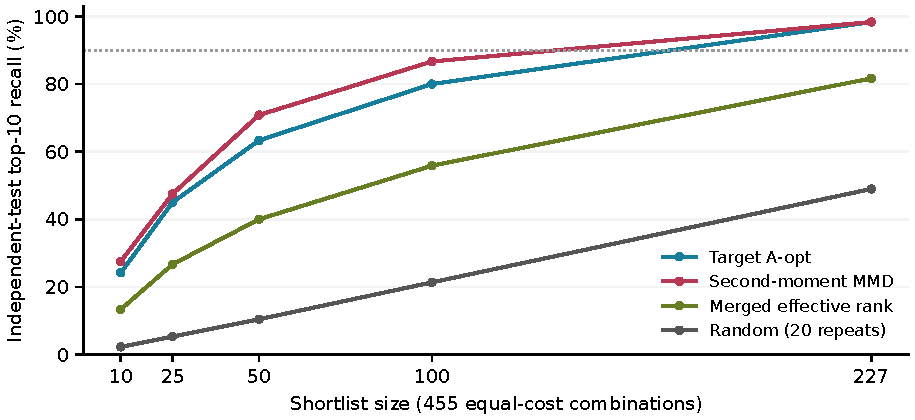
\includegraphics[width=\linewidth]{shortlist_recall.pdf}
\caption{由冻结结果表生成的 DomainNet 短名单规模曲线。虚线为预先指定的 $90\%$ 召回门槛。MMD 在更小短名单上平均召回更高，在主规模上与 A-opt 持平。曲线是描述性均值，不是方法间显著性检验。}
\label{fig:recall}
\end{figure}

这说明目标条件二阶信息对该短名单协议有用，但不能说明逆协方差加权必不可少：相同特征权限下，直接矩匹配也具有竞争力。同时，这不能证明相对 PACS/Office-Home 的改善由增加候选异质性引起。数据集、投影维度、样本预算和候选构造同时改变，尚未进行独立的异质性干预。

\subsection{低遗憾与有效区间可能不具信息量}
事后诊断表明，十二个 DomainNet 任务的完整相对 Brier 跨度 $[\max_S b(S)-\min_S b(S)]/|\min_S b(S)|$ 为 $0.0280\%$ 至 $0.4242\%$。因此，无论筛选方式如何，\emph{每一个}候选都满足 $5\%$ 遗憾门槛。通过这个子门控在此不具有区分作用。主结果中有意义的证据是固定评价次数下保留高排名候选；但精确前十名成员也可能对有限测试集上的微小差异敏感。

\begin{figure}[t]
\centering
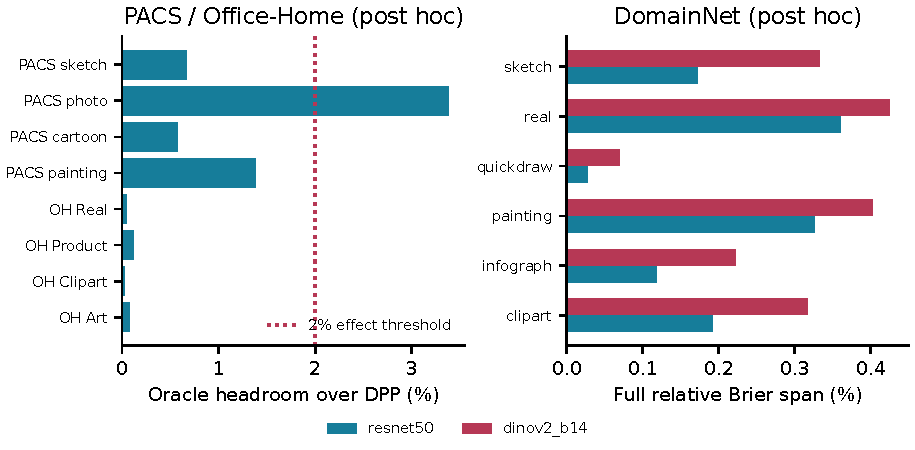
\includegraphics[width=\linewidth]{headroom_diagnostics.pdf}
\caption{不改变冻结门控的事后诊断。左：八个 PACS/Office-Home 目标单位的 oracle 相对 DPP 改善空间，先平均编码器。右：DomainNet 任务内部最好与最坏组合的相对 Brier 跨度；所有柱均低于 $0.425\%$，远低于 $5\%$ 遗憾门槛。两个面板回答不同问题，不能直接比较为同一种效应量。}
\label{fig:diagnostics}
\end{figure}

不同组合的准确率存在变化，其 oracle 与 Brier oracle 不总一致。因此不能把低 Brier 遗憾描述为一般分类性能保持。读出器对 one-hot 岭回归分数施加固定温度 softmax，校准与分数尺度可能促成微小 Brier 差异，但当前实验尚未证明该机制。评价前十名稳定性还需要重复独立测试或逐样本配对重采样，本文不声称已经完成。

压缩证书体现出类似区别。早期四编码器谱秩扫描中，全部 2,880 个已选择前缀的区间覆盖其精确分数，但在秩至多 50 的 7,200 个贪心步骤中，没有一步被认证。另一项包含 20 个种子、1,440 个配置的目标风险草图实验也未通过字节预算门控：在覆盖完整网格且平均使用至多四分之一紧凑 Full-Gram 字节的策略中，与 Full-Gram 贪心所选集合的最佳一致率仅为 $15.42\%$，对应成对比较证书率 $3.91\%$。覆盖率是正确性检查，不足以证明决策有效或实际通信节省（附录\ref{app:diagnostics}）。

\section{讨论与结论}
\label{sec:conclusion}
现有证据区分三类主张。Gram 可加性及满足相容条件的局部谱计算，是精确代数陈述；目标加权 A-optimal 风险由共享贝叶斯线性模型支持；真实分类中的有效短名单预筛选，则仍是候选族、读出器、目标样本与工作点共同决定的经验性质。这些推论不能任意逆转或推广。

在已审计的等成本 DomainNet 构造中，以约一半评价次数，目标二阶几何比已测目标无关多样性规则保留明显更多的测试前十名候选。最简单的成功同信息规则，即二阶矩 MMD，与 A-opt 对该结论同样重要。PACS/Office-Home 失败、有限 oracle 改善空间、宽松遗憾门控及较弱的压缩决策能力，都阻止我们作出更广泛的效用或优越性主张。

主要限制是仅一个新的等成本数据集、六个相关目标单位、一个固定投影种子、一种线性读出器，以及缺乏端到端时间收益的独立证据。下一步需要独立等成本数据集、主指标和前十名集合的稳定性检验、匹配的总成本测量，以及受控检验逆协方差加权何时比矩匹配更有价值。在这些检验完成前，特征几何应被理解为有条件的预筛选信号，仍需后续标签验证和明确的失败诊断。

\label{main-text-end}
\clearpage
\subsection*{AI 使用声明}
生成式 AI 工具参与了概念重构、数学命题与证明草拟、实验设计、软件实现、结果解释、文献检索、论文写作、绘图脚本编写及中文翻译。本稿数值发现来自已记录的实验产物，而非生成的观测值。AI 辅助不构成对实验产物或数学主张的独立验证。提交版本的最终核验与责任仍由人类作者承担。

\subsection*{可复现性声明}
附录\ref{app:proofs} 给出证明细节；第\ref{sec:protocol}节和附录\ref{app:protocol} 给出预处理、访问规则、候选构造、指标与结果路径。代码仓库为 \url{https://anonymous.4open.science/r/collapsemodel-1DB6}。结果表和 manifest 支持汇总复现；大型特征缓存通过哈希标识，不重复存入 Git。我们不声称不同硬件能够逐位复现全部特征。

\subsection*{伦理声明}
研究使用既有基准图像及预训练编码器，不新增参与者招募。公开可用并不消除图像许可、隐私或表示偏差问题。我们不声称多样的特征谱或高短名单召回率意味着所选数据池在社会层面具有代表性、公平性或隐私保护。候选类别体系、预训练重叠不确定性及视觉分类限制了下游部署主张。数据集和模型访问仍须遵守其原有条款。

\bibliography{references}
\bibliographystyle{iclr2027_conference}
\clearpage
\appendix
\section{证明与数学主张的适用范围}
\label{app:proofs}
设 $u,v$ 为单位方向，$u^\top v=c\in[0,1]$。在正交基 $u,z$ 中写成 $v=cu+\sqrt{1-c^2}z$，算子 $a^2uu^\top+b^2vv^\top$ 表示为
\begin{equation}
 \begin{pmatrix}
 a^2+b^2c^2 & b^2c\sqrt{1-c^2}\\
 b^2c\sqrt{1-c^2} & b^2(1-c^2)
 \end{pmatrix}.
\end{equation}
其迹为 $a^2+b^2$，行列式为 $a^2b^2(1-c^2)$，因此特征值为
\begin{equation}
 \lambda_{\pm}=\frac{a^2+b^2\pm\sqrt{(a^2-b^2)^2+4a^2b^2c^2}}{2}.
 \label{eq:local}
\end{equation}
当 $c=1$ 时，第二分支为零。若相关子块相互正交，且对两个源 Gram 都是不变子空间，汇集这些特征值对便得到完整谱；未配对方向贡献自身特征值。这一相容条件不可省略，因为主向量不必是奇异向量。

固定 $H_S$ 并采用高斯似然，对先验与似然乘积完成平方可得后验精度 $P_0^{-1}+\sigma^{-2}H_S^\top H_S$ 和均值 $\mu_S=P_S\sigma^{-2}H_S^\top y_S$。对独立目标观测 $y=h^\top\theta+\epsilon$，给定训练数据与 $h$，有
\begin{equation}
 \E[(y-h^\top\mu_S)^2\mid H_S,y_S,h]=\sigma^2+h^\top P_Sh.
\end{equation}
对 $h$ 积分得到式\eqref{eq:risk}。这里假设目标协变量分布不会在该模型之外额外透露关于 $\theta$ 的信息。若源数据具有不同回归函数，或标签为多分类且采用 softmax 读出，则该推导不再等于所评价的损失。证明不约束这种模型误设误差。以有限样本估计替代 $C_T$ 还引入另一类偏差，恒等式也不会自动消除它。

若 $G\succeq\widetilde G\succeq0$，逆矩阵序给出 $(P_0^{-1}+\sigma^{-2}G)^{-1}\preceq(P_0^{-1}+\sigma^{-2}\widetilde G)^{-1}$。与 PSD 目标矩相乘取迹保持该顺序。更一般地，若遗漏草图尾部之和满足 $0\preceq G-\widetilde G\preceq\delta I$，定义 $B=P_0^{-1}+\sigma^{-2}\widetilde G$，则
\begin{equation}
 \tr\!\left(\widehat C_T(B+\sigma^{-2}\delta I)^{-1}\right)
 \leq f_A(G)\leq\tr(\widehat C_TB^{-1}).
 \label{eq:interval}
\end{equation}
各 PSD 尾部的有效谱范数上界之和，是一种可取的 $\delta$。当某候选上界低于所有竞争者下界时，可以认证该候选的代理排序。因此，除了覆盖率，区间宽度也决定草图能否支撑下一次选择。归档扫描使用其文档中的字节计数，评价这类代理比较。

令 $S_Q$ 在 $\cQ_s$ 中最小化 $\ell$。短名单上的一致偏差给出
\begin{equation}
 \ell(\widehat S)\leq v(\widehat S)+\varepsilon
 \leq v(S_Q)+\varepsilon\leq\ell(S_Q)+2\varepsilon.
\end{equation}
减去 $\min_{S\in\cC}\ell(S)$ 即得式\eqref{eq:decomposition}。该代数推导没有给出概率声明。若要获得总体泛化保证，必须结合真实依赖与选择流程另外证明偏差事件。有限测试集上的穷举分数本身不足以提供这种证明。

映射 $\phi(h)=hh^\top$ 采用 Frobenius 内积，满足 $\langle\phi(h),\phi(h')\rangle_F=(h^\top h')^2$。源与目标经验特征均值之间的平方距离即式\eqref{eq:mmd}。这是有偏经验平方 MMD，即 V 统计量，而非去掉对角项的无偏估计。它依赖非中心化二阶矩，无法区分所有具有相同二阶矩的分布。我们将其作为计算简单的同信息对照，而非完备分布差异度量。

\section{实现与审计细节}
\label{app:protocol}
原 DomainNet 实验拟合岭回归读出，并将其分数转换为类别概率。权重与 Brier 损失为
\begin{equation}
 \begin{aligned}
 W_S&=(I+G_S)^{-1}\sum_{i\in S}H_i^\top Y_i,\qquad
 p(x)=\operatorname{softmax}(h(x)^\top W_S),\\
 b(S)&=\frac1{n_T}\sum_t\norm{p(x_t)-e_{y_t}}_2^2.
 \end{aligned}
\end{equation}
$Y_i$ 为固定 100 类词表下的源 one-hot 标签矩阵。不使用截距或温度调参。载入 float32 特征后，线性代数以 float64 计算。通过 Gram 特征分解计算有效秩时，先将负舍入特征值裁剪为零，再取平方根得到奇异值，仅保留 $\sigma_j>\sigma_{\max}\sqrt{8\epsilon_{64}\max(n_S,d,1)}$。代码对零矩阵返回零秩。该阈值针对数值秩，不改变熵定义。共享投影种子为 $20260911$，维度为 $128$；冻结 DomainNet 协议内部没有根据结果选择维度。

Bayesian D-opt 最大化 $\log\det(I+G_S)$。子空间 DPP 取每个块的前 16 个 Gram 特征向量 $U_i$，定义 $K_{ij}=\norm{U_i^\top U_j}_F^2/16$、$K_{ii}=1$，将其数值投影到 PSD 相关矩阵，再最大化 $\log\det(K_{S,S}+10^{-8}I)$。该核描述块子空间，而非单图像特征。域平衡最大化已覆盖域数量，减去各域块数平方和的 $10^{-3}$ 倍。确定性分数按组合标识字典序处理并列。这些是固定对照；该 DPP 构造表现不佳，不是对所有行列式选择方法的结论。

DomainNet 记录图像内容哈希、样本标识、官方划分、角色及类别词表。特征提取前验证归档与划分校验和。角色互斥和重复内容检查处理已物化基准内部的重叠，但不能排除语义近重复或预训练污染。全部筛选方法使用相同源块、投影、目标选择行和候选集合。特征提取忽略标签，基准物化则使用类别元数据，并为后续授权阶段存储标签。

筛选、验证与审计 manifest 绑定配置和上游产物哈希，分阶段加载器执行标签与划分权限。原协议的验证阶段单独评价每种方法或随机重复。选择冻结后，测试审计覆盖每个编码器的全部 $6\times455$ 个组合，穷举 oracle 作为研究参照。补实验的缓存策略如下。

CUDA 重建保留原样本标识、候选成员、预处理和超参数，全部十二个 Brier 前十名集合与原实验一致。逐样本损失均值与重建聚合审计的误差不超过 $1.78\times10^{-15}$。每个目标域对其 2,048 个测试样本执行 2,000 次配对 bootstrap，全部组合、编码器和四种损失共享权重。拟合模型与验证选择固定，平局按组合标识处理。这些重采样衡量对测试样本抽取的敏感性。原 Brier 前十名与 NLL、原始平方损失及分类错误率前十名的平均重叠分别为 $\BrierNLLOverlap\%$、$\BrierSquaredOverlap\%$ 和 $\BrierErrorOverlap\%$。

种子 $20260917$、$20260918$、$20260919$、$20260920$ 生成新的 128 维 Rademacher 投影，保持投影前后行归一化。种子 $20260911$ 用作实现对照，不计入新种子均值。逻辑回归采用 L2 正则化、$C=1$、无截距、LBFGS，容差为 $10^{-6}$，最多迭代 1,000 次。若出现收敛警告则终止任务；实际没有出现警告，最大迭代次数为 24。类别词表固定，源数据中缺失类别的概率设为零。

所有方法保留原筛选规则、候选组合和五种短名单规模，由独立进程依次筛选、拟合验证、测试冻结模型。测试特征读取前，核验源码、配置、来源、模型及选择的哈希。每个读出器对全部组合拟合一次，各方法复用这些拟合结果。这种缓存穷举评价用于比较不同短名单的反事实结果。Brier、NLL 和错误率分别使用自己的验证损失作最终选择。原种子岭回归在 5,460 个重建测试组合上的最大损失差异为 $1.78\times10^{-15}$，全部 1,620 个 Brier 验证选择完全一致。

两个编码器、五个种子、两种读出器合计完成 54,600 次拟合。新种子汇总先在任务内平均随机重复，再在目标域内平均编码器和种子，最后平均六个域。每个读出器包含 48 个编码器--种子--目标域重复测量，但仍是共享相同源池的六个目标域单位。

归档保留历史实验编号用于定位结果，不应将其与论文科学问题混淆。以下路径相对于匿名代码仓库：
\begin{itemize}
\item 共享模型与偏移研究（E1）：\path{results/target_conditioned/e1_synthetic/expanded_v3_controlled_rng/}。
\item PACS/Office-Home 对照（E2）：\path{results/target_conditioned/e2_dataset_selection/method_v1/}。
\item 事后改善空间（E2a）：\path{results/target_conditioned/e2_dataset_selection/oracle_headroom_v1/}。
\item 等成本短名单（E2b）：\path{results/target_conditioned/e2b_fixed_cost_shortlist/domainnet_v1/}。
\item 风险草图扫描（E5）：\path{results/target_conditioned/e5_sketch_certificate/expanded_v3_controlled_rng/}。
\item 重建与测试重采样（R1/R2）：\path{results/target_conditioned/revision_20260916/}。
\item 投影与读出器补实验（R3/R4）：\path{results/target_conditioned/revision_20260917/}。
\end{itemize}
{\raggedright
DomainNet 数据 manifest 前缀为 \texttt{1ba25059df70be4d}，候选集 ID 前缀为 \texttt{545fe86c8c9e8304}，汇总 ID 前缀为 \texttt{2d473cb9eb977e85}；完整 SHA-256 位于产物中。原配置为 \path{code/configs/target_conditioned_e2b/domainnet_v1.json}，实现为 \path{scripts/run_target_conditioned_e2b_shortlist.py}。补实验采用 \path{code/configs/target_conditioned_e2b/readout_projection_v1.json} 和 \path{scripts/run_e2b_readout_projection.py}，汇总表位于 R3/R4 目录内的 \path{revision_results/e2b_readout_projection_v1/summary/}。论文的 \path{build_assets.py} 从记录的源文件生成表格、图、数字宏和双语摘要，完整输入哈希记入 \path{generated/asset_manifest.json}。\par}

三份原始特征矩阵未重复存入 Git。元数据记录精确文件哈希、检查点哈希、形状、预处理、提取代码版本和运行环境。重新提取需要原始公开数据及模型权重，不假设不同硬件逐位一致。仓库保留 manifest 和足够的结果表，可在没有这些矩阵时复现报告的汇总结果。

\section{补充结果}
\label{app:diagnostics}
PACS/Office-Home、$K=3$ 时，A-opt 平均 Brier 为 $0.826769$，DPP 为 $0.829162$，MMD 为 $0.828719$。A-opt 减去基线的配对区间分别为 $[-0.007449,0.000731]$ 和 $[-0.003392,-0.000712]$。事后审计覆盖每个任务全部 220 个组合。Oracle 相对 DPP 的改善空间描述性 95\% 区间为 $[0.162,1.617]\%$；仅 PACS photo 在目标单位层面超过原 $2\%$ 门槛。相对父方法的事后测试最优包络，oracle 平均还能改善 $0.087\%$。该包络是基于结果的参照，不是可用于选择的基线。

表\ref{app:readout-table} 给出主规模下完整的 Brier 召回比较。A-opt 和 MMD 平均相对选择遗憾相同：岭回归为 $\RidgeSelectedRegret\%$，逻辑回归为 $\LogisticSelectedRegret\%$。两者全部新种子主设置 Brier 短名单均包含经验 oracle。

\begin{table}[ht]
\centering
\caption{表中报告全部补实验评分规则在 $s=227$ 时的 Brier 前十名召回率（\%）。平均方式与表\ref{tab:readout} 相同，不包括原种子对照。}
\label{app:readout-table}
\begin{tabular}{lrr}
\toprule
Screen & Ridge & Logistic\\
\midrule
Target A-opt & 98.33 & 98.33 \\
Second-moment MMD & 99.38 & 98.96 \\
Bayesian D-opt & 82.29 & 86.46 \\
Merged effective rank & 80.42 & 85.42 \\
Random (20 repeats) & 50.12 & 48.97 \\
Target energy & 41.04 & 33.96 \\
DPP subspace & 28.75 & 35.42 \\
Domain balance & 26.46 & 31.67 \\
\bottomrule
\end{tabular}

\end{table}

A-opt 最低分类错误率召回出现在 DINOv2、Quickdraw、逻辑回归、投影种子 $20260918$ 的任务中。测试错误率 oracle 为 $85.9863\%$，验证选择为 $87.6465\%$。虽然前十名召回只有 $\WorstErrorRecall\%$，短名单仍保留 oracle。因此，保留最佳成员与保留前十名回答不同问题，二者也都不同于可用模型的绝对质量。

四编码器、十个构造种子的谱扫描使用六个重叠设置和四种预算，每个草图秩有 960 个配置。秩为 $10,20,50$ 时，相对仅使用秩的对照，Gram 草图在精确合并有效秩上的收益分别为 $2.09,3.81,4.94\%$，DPP 为 $4.90,5.48,5.68\%$。这些是几何目标收益，不是分类准确率。熵连续性界采用\citet{audenaert2007} 这一类型的界；2,880 个已选择前缀区间全部覆盖，但 7,200 个评价的贪心步骤没有一步得到认证。结果来源为 \path{results/two_stage_controlled_rank_sweep_corrected_v3/}。这并不意味着所有低秩草图都必然失败。

独立 E5 研究将草图载荷与紧凑对称 float64 Gram 比较，而非与更大的稠密存储比较。在覆盖完整网格、平均字节比不超过 $25\%$ 的策略中，与 Full-Gram 贪心的最佳所选集合一致率为 $15.42\%$，由自适应秩上限 2 获得，平均字节比为 $14.91\%$。其成对证书率为 $3.91\%$，完整选择认证率为零。自适应回退能够实现完全所选集合一致，但计入此前传输后，平均成本约为紧凑 Gram 字节的 $160\%$，未达到决策与通信的联合要求。参照是 Full-Gram 贪心，而非穷举全局最小解。

另一项早期实验在 21 个来源上训练源监督 bottleneck adapter，使用四个编码器、五个 adapter 种子审计七个目标。目标训练内验证采用三个分层五折划分，选择冻结后独立读取 held-out 目标测试集。冻结 identity 平均准确率为 $0.83654$，未训练随机 adapter 为 $0.77144$，验证 oracle 源监督 adapter 为 $0.76951$。后者比 identity 低 $0.06703$，目标聚类 95\% 区间为 $[-0.09771,-0.04400]$。相对该 adapter 族的小短名单遗憾因而不代表下游收益。这不是 DomainNet 实验，也不是对所有适应方法的否定。结果位于 \path{results/two_stage_repeated_cv_utility_corrected_v3/}。

\end{document}
